
\subsection{Appendix A. How the filters alter the signal}
\label{Apx:A}

\begin{figure}[H]
    \centering
    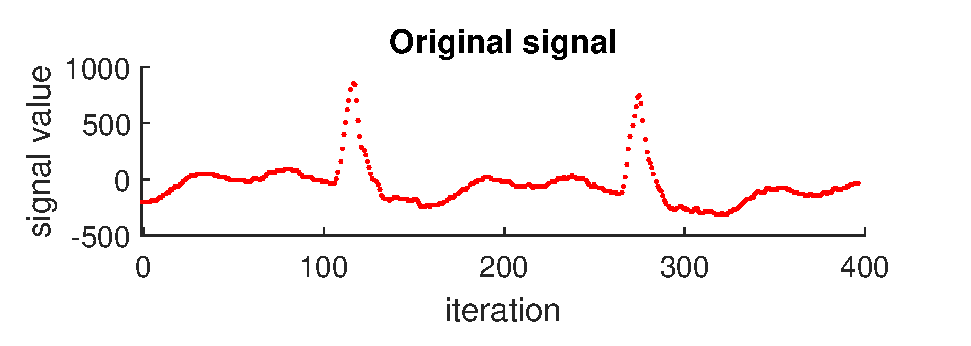
\includegraphics[width=1.0\textwidth]{Appendix/fig/1original.eps}
    \caption{Signal as a function of iteration.}
    \label{fig:1original}
\end{figure}

\begin{figure}[H]
    \centering
    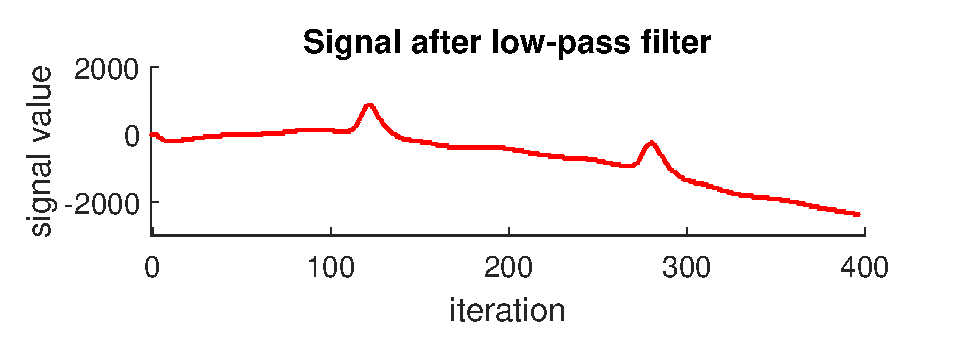
\includegraphics[width=1.0\textwidth]{Appendix/fig/2afterLowPass.eps}
    \caption{Signal as a function of iteration.}
    \label{fig:2afterLowPass}
\end{figure}

\begin{figure}[H]
    \centering
    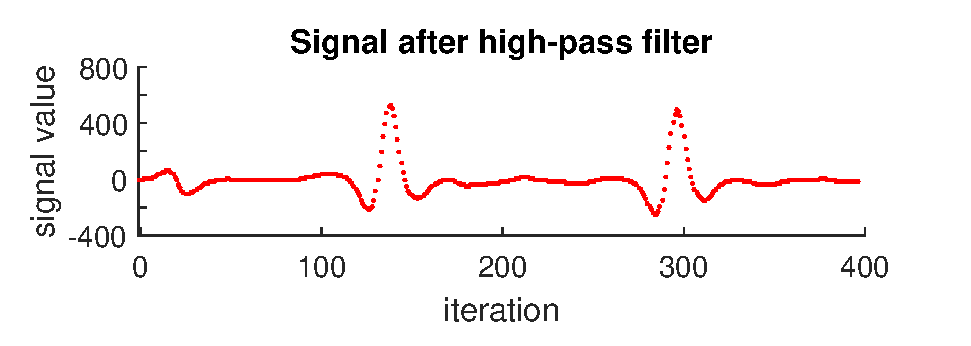
\includegraphics[width=1.0\textwidth]{Appendix/fig/3afterHighPass.eps}
    \caption{Signal as a function of iteration.}
    \label{fig:3afterHighPass}
\end{figure}

\begin{figure}[H]
    \centering
    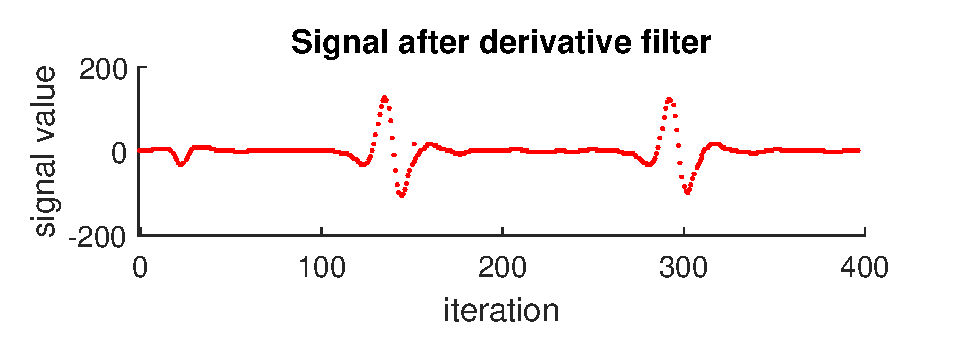
\includegraphics[width=1.0\textwidth]{Appendix/fig/4afterDerivative.eps}
    \caption{Signal as a function of iteration.}
    \label{fig:4afterDerivative}
\end{figure}

\begin{figure}[H]
    \centering
    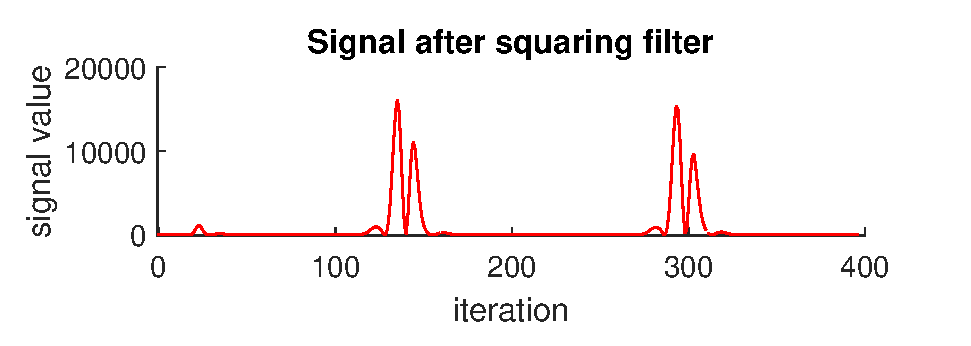
\includegraphics[width=1.0\textwidth]{Appendix/fig/5afterSquaring.eps}
    \caption{Signal as a function of iteration.}
    \label{fig:5afterSquaring}
\end{figure}


\begin{figure}[H]
    \centering
    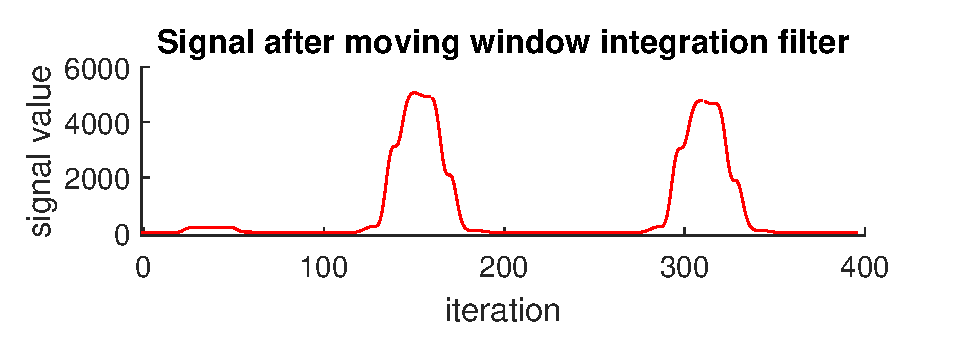
\includegraphics[width=1.0\textwidth]{Appendix/fig/6afterMovInt.eps}
    \caption{Signal as a function of iteration.}
    \label{fig:6afterMovInt}
\end{figure}


